\subsubsection{Architecture}

\begin{figure}[!htb]
  \centering
  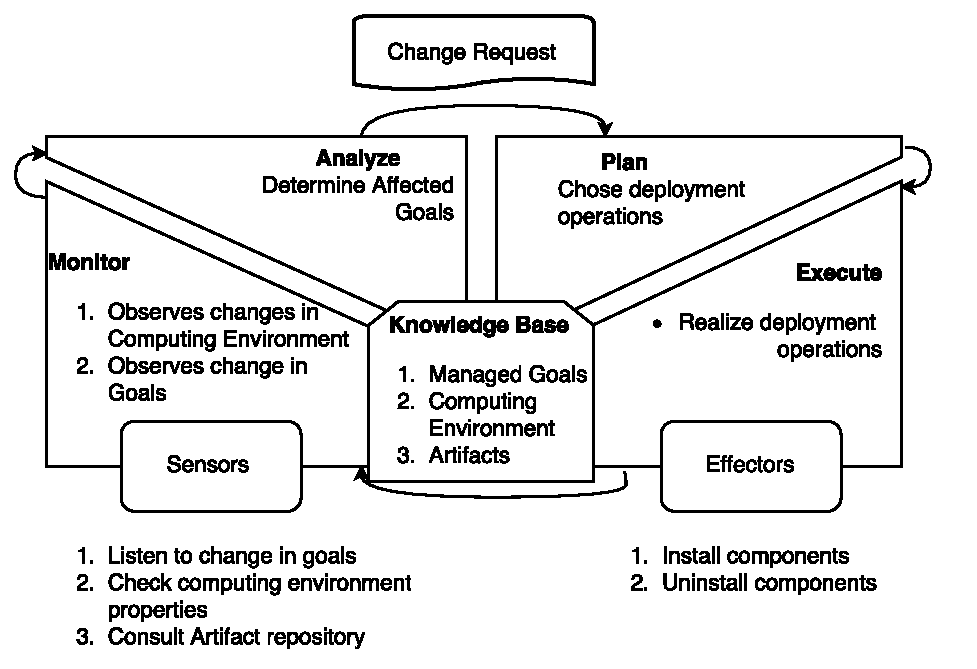
\includegraphics[width=\linewidth]{goald_mape_k}
  \caption{Goald Deployment Manager}
\label{fig:goald_mape_k}
\end{figure}

\begin{itemize}
  \item events: are handled to registered listeners.
\end{itemize}

\subsubsection{Knowledge Base}

The knowledge base store a model of goals the system much achieve, the computing environment context and current deployed artifacts.

The information in the knowledge base can be of two types:
\begin{itemize}
  \item facts: can be queried about by registered components
\end{itemize}


\subsubsection{Monitors}

Monitors are components that observes changes in the goals and context. All
\begin{itemize}
  \item Goal Change Monitor is responsible for listening to request of include or remove goals.
  \item Computing Environment monitor is responsible to verify \emph{facts} about the computing enivronment as introduced in~\ref{context}. \emph{Facts} are stored in the Knowledge Base and used to evaluate context conditions.
  \item Repository monitors observe changes in software repositories.
  \item Introspective monitors observe the system state and behavior. (ex: monitor that check if there is any monitor that dispatches events that no one cares about)
\end{itemize}

The result of monitors can be:
\begin{itemize}
  \item Change the knowledge base
  \item Dispatch Events
\end{itemize}

Core Components:
\begin{itemize}
  \item Timer Monitoring Policy:
  \item Computing Environment Sensors: listen to timeouts of monitoring policy. Sense the environment. Update the knowledge base and dispatch events for changes in the environment.
  \item Goals change listeners: listen for external entities that want to change the goals of the machine. The interface is implementation dependent (e.g HTTP service, GUI, command line). Dispatch External Change Requests.
  \item Repository Monitor: queries repository for information about components.
\end{itemize}



\subsubsection{Analyzer}

Objective change analyzer

Computing environment change - evaluate if any system goal is affected.

Evaluate parametric formula for managed goals. If a goal probability of success drops below a threshold, dispatch deployment replanting event.

Handling evolution: simple approach favor a superior version.


\begin{itemize}
  \item Goals Change- Check if a goal request is a change request. A goal removal will affect another goals?

  \item Adaptation
In case of change in the available resources
it should be analyzed if the change threats the achievements of goals.

\end{itemize}

Listens to:
\begin{itemize}
  \item changes in the environment
  \item external changes in goals
\end{itemize}

Dispatch
\begin{itemize}
  \item Change Request: request a change in the deployment. Contains affected goals for what deployment should be replanned.
\end{itemize}

\subsubsection{Planner}

Receive change requests and enqueue it.

Deployment Change Planner is responsible for finding which operation should be executed in order to (1) make the active goals achievable. (2) Free up resource not associated with active goals.

How deployment is planned and the algorithm used will be described in Section~\ref{sec:deployment_planning}.

Components
\begin{itemize}
  \item Context Evaluation: it is responsible to evaluate if context conditions are satisfied for a given component in a given context.
\end{itemize}

Listens To:
\begin{itemize}
  \item Change Request
\end{itemize}

Dispatch:
\begin{itemize}
  \item Query Repositories: request information about available components that provide given goals.
  \item Execute Plan: request a deployment plan to be executed.
\end{itemize}



\subsubsection{Execute}

Executor components are responsible to actuate in the system.
Deployment Change Executor is responsible for get components from repository and execute deployment operations such as install and uninstall components.

% Fix Resource

% Change monitoring policy

Listen To:
\begin{itemize}
  \item Execute Plan:
\end{itemize}
